% Maerz 2015
% Autor: Mandy Vogel
% Tests 
\documentclass[xcolor={table}]{beamer}
\usetheme{Singapore}

%% \usepackage{listings}

\begin{document}

\title{Classical Tests}   
\author{Mandy Vogel} 
\date{\today}
%\logo{\includegraphics[scale=0.14]{PIC1}}

\begin{frame}
\titlepage
\end{frame}

\begin{frame}
\frametitle{Table of Contents}\tableofcontents
\end{frame}

\section{Preliminaries}
\subsection{Classifaction of tests}
\begin{frame}\frametitle{Tests}
  \begin{columns}
    \begin{column}{0.7\textwidth}
      \begin{itemize}
      \item<1->\textbf{Parametric classical tests}
        \begin{itemize}
        \item<4-> for central tendency
        \item<5-> for proportion
        \item<6-> for variability
        \item<7-> for distribution functions
        \item<8-> for association
        \end{itemize}
      \item<2->\textbf{Distribution-free tests}
        \begin{itemize}
        \item<4-> for central tendency
        \item<6-> for variability
        \item<7-> for distribution functions
        \item<8-> for association
        \end{itemize}
      \item<3->\textbf{Sequential tests}
        \begin{itemize}
        \item<4-> for central tendency
        \item<5-> for proportion
        \item<6-> for variability
        \end{itemize}
      \end{itemize}
    \end{column}
    \onslide<9->
    \begin{column}{0.3\textwidth}
      In each case:
      \begin{itemize}
        \item[]<9-> 1 sample
        \item[]<9-> 2 samples
        \item[]<9-> $k$ samples
      \end{itemize}
    \end{column}
  \end{columns}
\end{frame}

\begin{frame}\frametitle{four possible situations}\footnotesize
\begin{tabular}{cl|c|c|}
  &  \multicolumn{1}{c}{}& \multicolumn{2}{c}{\textbf{Situation}} \\
  &  \multicolumn{1}{c}{}& \multicolumn{1}{c}{$H_0$ is true} & \multicolumn{1}{c}{$H_0$ is false} \\
\cline{3-4}
\textbf{Conclusion} & $H_0$ is not rejected &  Correct decision  & Type II error \\
\cline{3-4}
 & $H_0$ is rejected & Type I error &  Correct decision  \\
\cline{3-4}
\end{tabular}
\end{frame}

\subsection{Common symbols}
\begin{frame}\frametitle{Common symbols}
  \rowcolors[]{1}{gray!10}{gray!30}
  \begin{tabular}{@{} >{\ttfamily}l l@{}} 
    \rowcolor{gray!40}symbol & meaning \onslide<2->\\
    $n$ & number of observations (sample size)\onslide<2->\\
    $K$ & number of samples (each having $n$ elements) \onslide<3->\\
    $\alpha$ & level of significance \onslide<3->\\
    $\nu$ & degrees of freedom \onslide<3->\\
    $\sigma$ & standard deviation (population)\onslide<3->\\
    $s$ & standard deviation (sample)\onslide<4->\\
    $\mu$ & population mean \onslide<4->\\
    $\bar{x}$ & sample mean \onslide<4->\\
    $\rho $ & population correlation coefficient \onslide<4->\\
    $r$ & sample correlation coefficient \onslide<5->\\
    $Z$ & standard normal deviate \\
  \end{tabular}
\end{frame}

\begin{frame}\frametitle{Alternatives}
    \only<1>{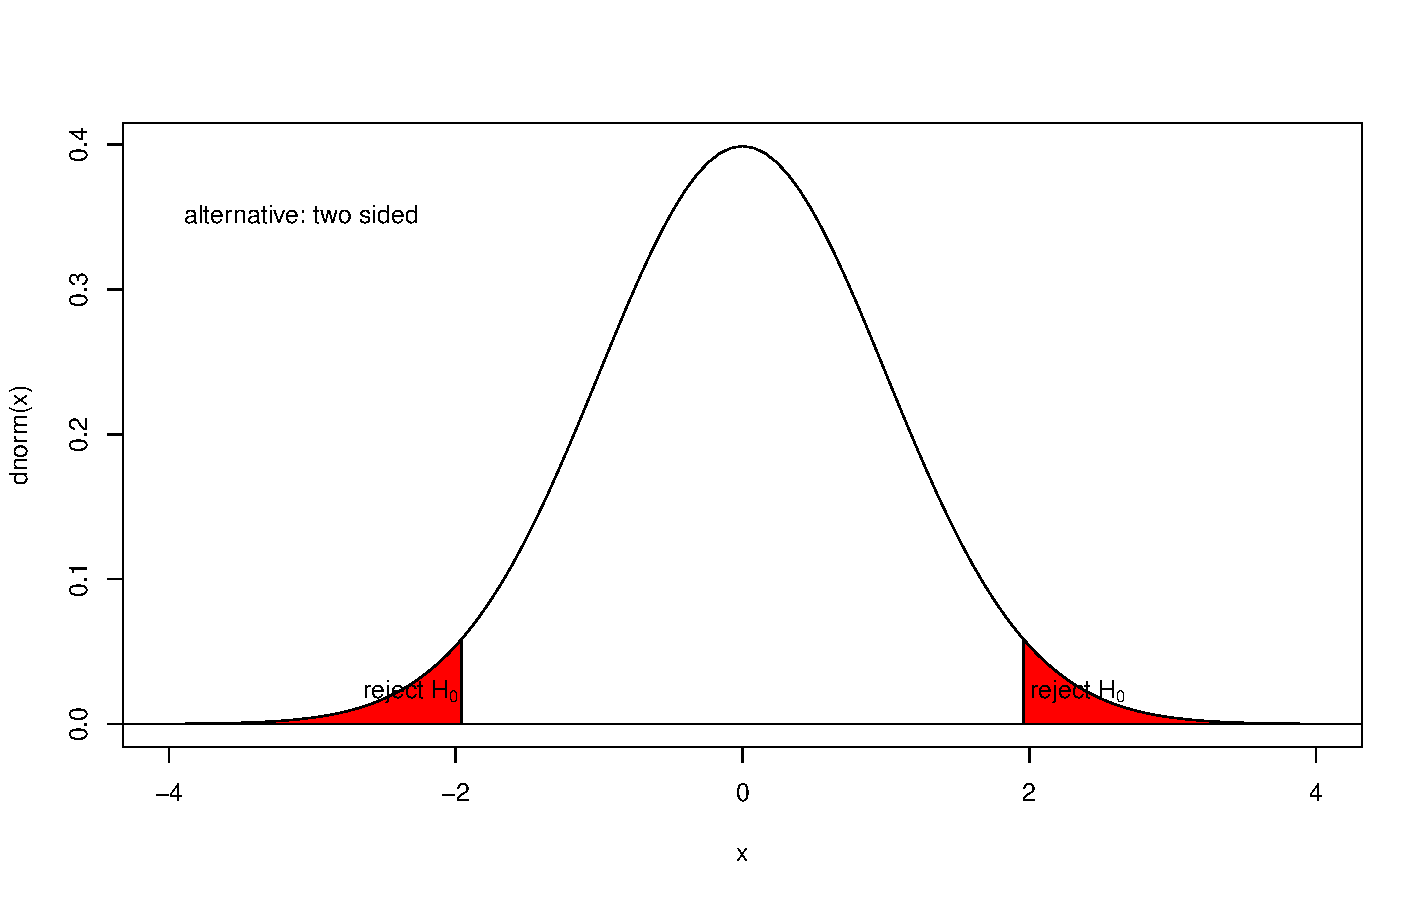
\includegraphics[width=11cm, height=7cm]{twosided.pdf}}
    \only<2>{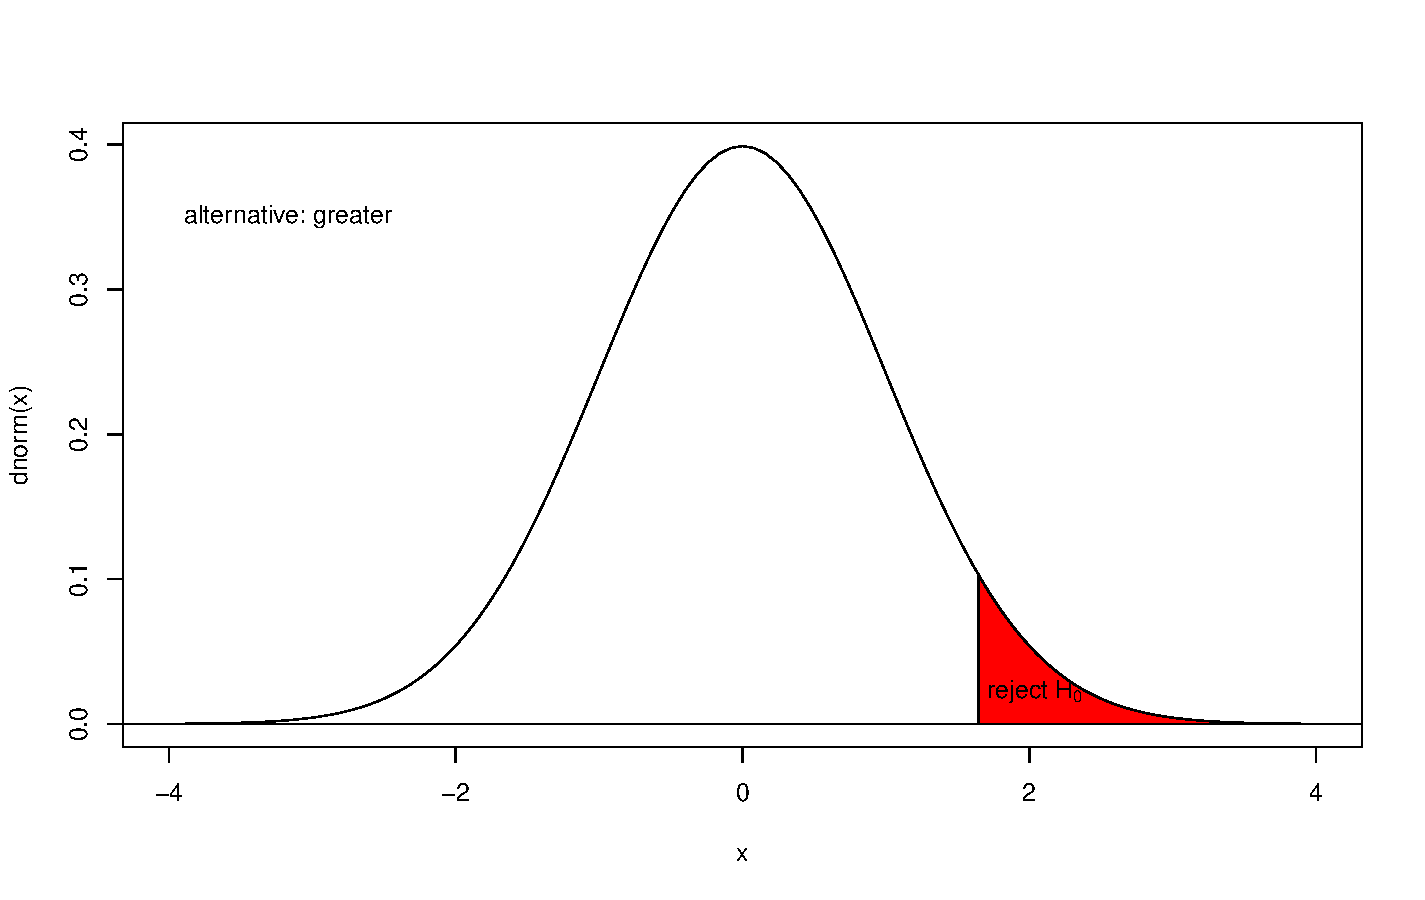
\includegraphics[width=11cm, height=7cm]{greater.pdf}}
    \only<3>{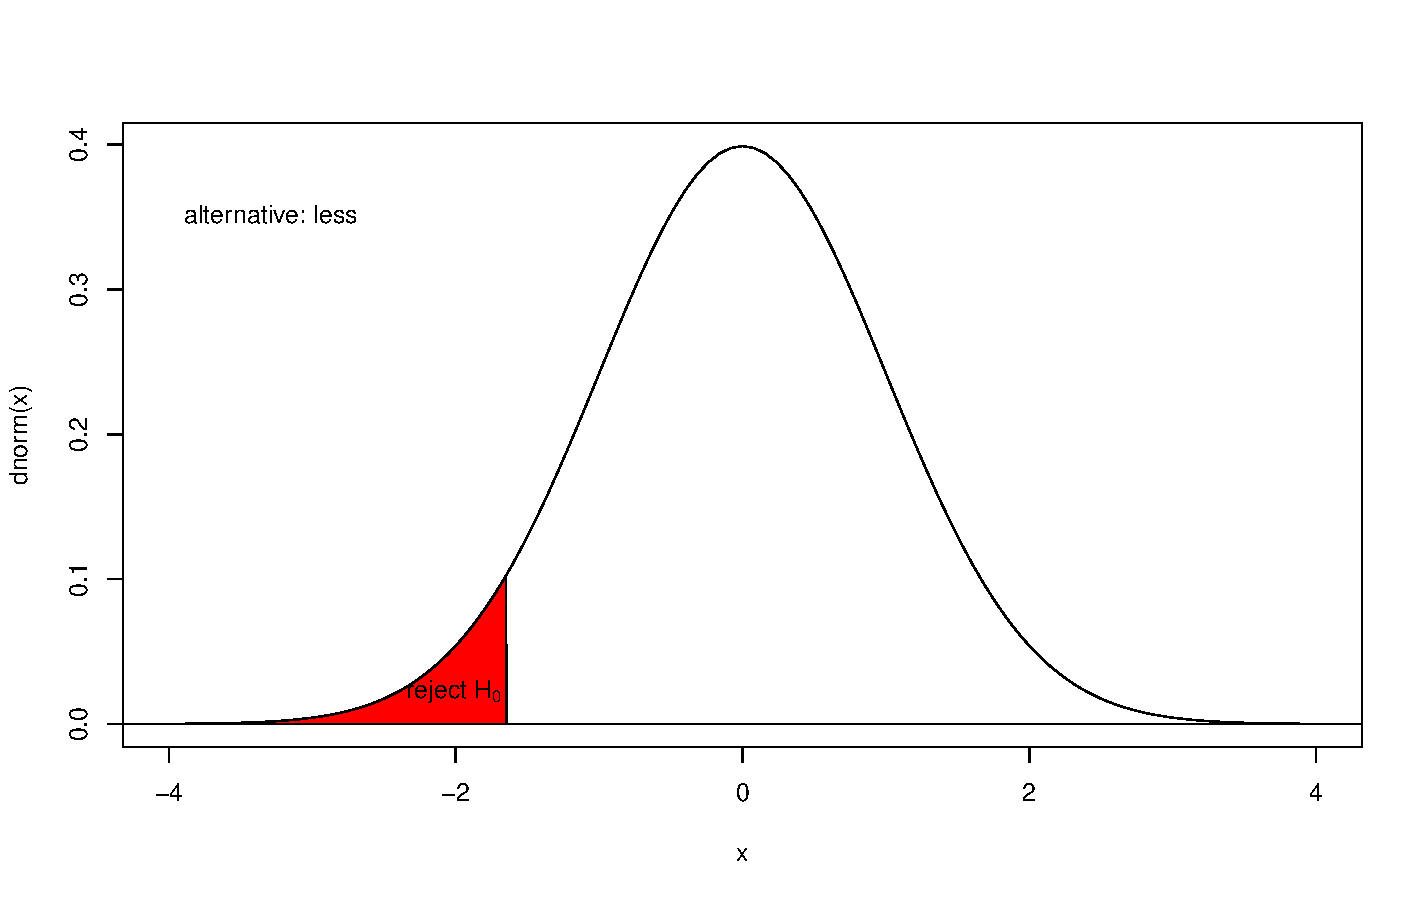
\includegraphics[width=11cm, height=7cm]{less.pdf}}
\end{frame}


\begin{frame}\frametitle{Alternatives}
  \begin{alertblock}{Note:}
    The p-value is the probability of the sample estimate (of the respective estimator) under the null.
  \end{alertblock}
\end{frame}

\section{Understand Hypothesis Tests}\small 
\subsection{Z-test}
\begin{frame}\frametitle{Z-test for a population mean} 
The z-test is a something like a t-test (it is like you would know almost everything about the perfect conditions. It uses the normal distribution as test statistic and is therefore a good example.
  \begin{block}{Objective}
    To investigate the significance of the difference between an assumed population mean $\mu_0$ and a sample mean $\bar{x}$.
  \end{block}
  \begin{alertblock}{Limitations}
    \begin{enumerate}
      \item It is necessary that the population variance $\sigma^2$ is known. 
      \item The test is accurate if the population is normally distributed. If the population is not normal, the test will still give an approximate guide.
    \end{enumerate}
  \end{alertblock}
\end{frame}


\begin{frame}[fragile]\frametitle{Z-test for a population mean}\footnotesize
    \begin{exampleblock}{Test statistic}
    $$Z = \frac{\bar{x}-\mu_0}{\sigma/\sqrt{n}}$$
  \end{exampleblock}
    \begin{enumerate}
    \item Write a function which takes a vector, the population standard deviation and the population mean as arguments and which gives the Z score as result. 
      \begin{itemize}
      \item name the function \texttt{ztest} or \texttt{my.z.test} - not \texttt{z.test} because \texttt{z.test} is already used
      \item set a default value for the population mean
      \end{itemize}
    \item add a line to your function that allows you to also process numeric vectors containing missing values!
    \item the function \texttt{pnorm(Z)} gives the probability of $x \leq Z $. Change your function so that it has the p-value (for a two sided test) as result. 
    \item now let the result be a named vector containing the estimated difference, Z, p and the n.
    \end{enumerate}
You can always test your function using simulated values: \texttt{rnorm(100,mean=0)} gives you a vector containing 100 normal distributed values with mean 0.
\end{frame}

\begin{frame}[fragile]\frametitle{Z-test for a population mean}
Write a function which takes a vector, the population standard deviation and the population mean as arguments and which gives the Z score as result.
\begin{verbatim}
> ztest <- function(x,x.sd,mu=0){
+     sqrt(length(x)) * (mean(x)-mu)/x.sd
+ }
> set.seed(1)
> ztest(rnorm(100),x.sd = 1)
[1] 1.088874
\end{verbatim}
\end{frame}

\begin{frame}[fragile]\frametitle{Z-test for a population mean}
Add a line to your function that allows you to also process numeric vectors containing missing values!
\begin{verbatim}
> ztest <- function(x,x.sd,mu=0){
+     x <- x[!is.na(x)]
+     if(length(x) < 3) stop("too few values in x")
+     sqrt(length(x)) * (mean(x)-mu)/x.sd
+ }
\end{verbatim}
\end{frame}

\begin{frame}[fragile]\frametitle{Z-test for a population mean}
The function \texttt{pnorm(Z)} gives the probability of $x \leq Z $. Change your function so that it has the p-value (for a two sided test) as result. 
\begin{verbatim}
> ztest <- function(x,x.sd,mu=0){
+     x <- x[!is.na(x)]
+     if(length(x) < 3) stop("too few values in x")
+     z <- sqrt(length(x)) * (mean(x)-mu)/x.sd
+     2*pnorm(-abs(z))
+ }
> set.seed(1)
> ztest(rnorm(100),x.sd = 1)
[1] 0.2762096
\end{verbatim}
\end{frame}


\begin{frame}[fragile]\frametitle{Z-test for a population mean}
Now let the result be a named vector containing the estimated difference, Z, p and the n.
\begin{verbatim}
> ztest <- function(x,x.sd,mu=0){
+     x <- x[!is.na(x)]
+     if(length(x) < 3) stop("too few values in x")
+     est.diff <- mean(x)-mu
+     z <- sqrt(length(x)) * (est.diff)/x.sd
+     round(c(diff=est.diff,Z=z,pval=2*pnorm(-abs(z)),n=length(x)),4)
+ }
> set.seed(1)
> ztest(rnorm(100),x.sd = 1)
    diff        Z     pval        n 
  0.1089   1.0889   0.2762 100.0000 

\end{verbatim}
\end{frame}

\begin{frame}\frametitle{Z-test for a population mean (3)} 
  \begin{block}{Variants}
    \begin{enumerate}
      \item Z-test for two population means (variances known and equal)
      \item Z-test for two population means (variances known and unequal)
    \end{enumerate}
    To investigate the statistical significance of the difference between an assumed population mean $\mu_0$ and a sample mean $\bar{x}$. There is a function \texttt{z.test()} in the \texttt{BSDA} package.
  \end{block}
  \begin{alertblock}{Limitations (again)}
    \begin{enumerate}
      \item It is necessary that the population variance $\sigma^2$ is known. 
      \item The test is accurate if the population is normally distributed. If the population is not normal, the test will still give an approximate guide.
    \end{enumerate}
  \end{alertblock}
\end{frame}

\section{t-Tests}
\subsection{One Sample t-test}
\defverbatim{\ttesta}{
\begin{verbatim}
> set.seed(1)
> x <- rnorm(12)
> t.test(x,mu=0) ## population mean 0

	One Sample t-test

data:  x
t = 1.1478, df = 11, p-value = 0.2754
alternative hypothesis: true mean is not equal to 0
95 percent confidence interval:
 -0.2464740  0.7837494
sample estimates:
mean of x 
0.2686377 
\end{verbatim}
}


\defverbatim{\ttestb}{
\begin{verbatim}


> t.test(x,mu=1) ## population mean 1

	One Sample t-test

data:  x
t = -3.125, df = 11, p-value = 0.009664
alternative hypothesis: true mean is not equal to 1
95 percent confidence interval:
 -0.2464740  0.7837494
sample estimates:
mean of x 
0.2686377 
\end{verbatim}
}

\begin{frame}[fragile]\frametitle{t-tests}
A t-test is any statistical hypothesis test in which the test statistic follows a \emph{Student's t distribution} if the null hypothesis is supported.
\begin{itemize}
\item \emph{one sample t-test}: test a sample mean against a population mean
$$ t = \frac{\bar{x}-\mu_0}{s/\sqrt{n}}$$ where $\bar{x}$ is the sample mean, $s$ is the sample standard deviation and $n$ is the sample size. The degrees of freedom used in this test is $n-1$
\end{itemize}
\end{frame}

\begin{frame}[fragile]\frametitle{One Sample t-test}
\only<1>{\ttesta}
\only<2>{\ttestb}
\end{frame}


\subsection{Two Sample t-tests}

\defverbatim{\ttestc}{

}

\begin{frame}[fragile]\frametitle{Two Sample t-tests}
There are two ways to perform a two sample t-test in R:
\begin{itemize}
\item given two vectors \texttt{x} and \texttt{y} containing the measurement values from the respective groups \texttt{t.test(x,y)}
\item given one vector \texttt{x} containing all the measurement values and one vector \texttt{g} containing the group membership \texttt{t.test(x ~ g)} (read: x dependend on g)
\end{itemize}
\end{frame}

\begin{frame}[fragile]\frametitle{Two Sample t-tests: two vector syntax}\footnotesize
\begin{verbatim}
> set.seed(1)
> x <- rnorm(12)
> y <- rnorm(12)
> g <- sample(c("A","B"),12,replace = T)
> t.test(x,y)

	Welch Two Sample t-test

data:  x and y
t = 0.5939, df = 20.012, p-value = 0.5592
alternative hypothesis: true difference in means is not equal to 0
95 percent confidence interval:
 -0.5966988  1.0717822
sample estimates:
 mean of x  mean of y 
0.26863768 0.03109602   
\end{verbatim}
\end{frame}


\begin{frame}[fragile]\frametitle{Two Sample t-tests: formula syntax}\footnotesize
\begin{verbatim}




> t.test(x ~ g)

	Welch Two Sample t-test

data:  x by g
t = -0.6644, df = 6.352, p-value = 0.5298
alternative hypothesis: true difference in means is not equal to 0
95 percent confidence interval:
 -1.6136329  0.9171702
sample estimates:
mean in group A mean in group B 
      0.1235413       0.4717726 
\end{verbatim}
\end{frame}


\begin{frame}[fragile]\frametitle{Welch/Satterthwaite vs. Student}
  \begin{itemize}
  \item if not stated otherwise \texttt{t.test()} will not assume that the variances in the both groups are equal
  \item if one knows that both populations have the same variance set the \texttt{var.equal} argument to TRUE to perform a student's t-test
  \end{itemize}
\end{frame}

\begin{frame}[fragile]\frametitle{Student's t-test}
\begin{verbatim}



> t.test(x, y, var.equal = T)

	Two Sample t-test

data:  x and y
t = 0.5939, df = 22, p-value = 0.5586
alternative hypothesis: true difference in means is not equal to 0
95 percent confidence interval:
 -0.5918964  1.0669797
sample estimates:
 mean of x  mean of y 
0.26863768 0.03109602   
\end{verbatim}
\end{frame}

\begin{frame}[fragile]\frametitle{t-test}
  \begin{itemize}
  \item the t-test, especially the Welch test is appropriate whenever the values are normally distributed
  \item it is also recommended for group sizes $\geq 30$ (robust against deviation from normality)
  \end{itemize}
\end{frame}

\end{document}
